\documentclass[a4paper,12pt,english]{article}
% *** LANGUAGE PACKAGES ***
\usepackage{babel}
\usepackage[utf8]{}
\usepackage[T1]{fontenc}
\usepackage{csquotes}
\usepackage{lmodern}		% Great font
\renewcommand*\familydefault{\sfdefault}
\usepackage[useregional]{datetime2}		% To use several date formats
\usepackage{textcomp, gensymb}
\usepackage{ragged2e}
\usepackage{multicol}
\setlength{\columnsep}{0.5cm}
\setlength{\parindent}{0pt}
\usepackage[dvipsnames,table]{xcolor}


% *** GEOMETRY PACKAGES ***
\usepackage{geometry}
\geometry{left=25mm,
	right=25mm,
	top=35mm,
	bottom=30mm,
	headheight = 35 mm
} 
\usepackage{lastpage}

% *** COLOR PACKAGES ***
\usepackage[most]{tcolorbox}
% Color definitions
\definecolor{blue}{RGB}{0,89,140}
\definecolor{gray}{RGB}{242,242,242}
\definecolor{grayblack}{RGB}{50,50,50}
\definecolor{blue2}{RGB}{10,62,157}
\definecolor{red2}{RGB}{173,17,0}
\definecolor{gray2}{RGB}{230,230,230}
\definecolor{mauve}{rgb}{0.58,0,0.82}
\definecolor{dkgreen}{rgb}{0,0.6,0}

% *** GRAPHICS RELATED PACKAGES ***
\usepackage{graphicx}       % Loading images
\usepackage{float}          % Figures inside minipages
\usepackage{wrapfig}		% Text wrapped around figure
\usepackage{tikz}			% Used to load cover figure
\usepackage{pgfplots}
\pgfplotsset{compat=1.18}

\usepackage[hypcap,font={color=grayblack}]{caption} % used to style the captions
\usepackage{subcaption} 	% For subfigures
\usepackage{overpic}		% To add text over figures
\graphicspath{{images/}}  % Figures relative directory

% *** HEADING AND FOOTER ***
\usepackage{fancyhdr} % For heading and footers
\renewcommand{\headrulewidth}{0.5pt}
\let\oldheadrule\headrule% Copy \headrule into \oldheadrule
\renewcommand{\headrule}{\color{grayblack}\oldheadrule}% Add colour to \headrule
\renewcommand{\footrulewidth}{0.5pt} 
\let\oldfootrule\footrule%
\renewcommand{\footrule}{\color{grayblack}\oldfootrule}% Add colour to \headrule
\pagestyle{fancy}                    % Default page style
\cfoot{}                             % Empty foot center  
\lhead{
\includegraphics[scale=0.1]{QubeCL_Logo.pdf}}     
\rhead{\textcolor{grayblack}{\small \AppNoteNumber}}        
%\lfoot{\textcolor{grayblack}{\DTMsetstyle{ddmmyyyy} \date}}
\lfoot{\textcolor{grayblack}{Revision \vhCurrentVersion}}
\rfoot{\textcolor{grayblack}{\small Pag. \thepage\ - \pageref*{LastPage}}} 			     % Total of pages



% *** TITLE PACKAGES ***
\usepackage{titlesec}
\titleformat{\section}{\color{grayblack}\normalfont\Large\bfseries}{\thesection}{1em}{}
\titleformat{\subsection}{\color{grayblack}\normalfont\large\bfseries}{\thesubsection}{1em}{}
\usepackage{setspace} % Para ajustar la separación entre líneas del documento

% *** TABLE PACKAGES ***
\usepackage{booktabs}
\usepackage{colortbl}
\usepackage{footnote} % To have footnotes inside tables
\usepackage{array}
\usepackage{multirow}
\usepackage{longtable}
\usepackage{arydshln}

\usepackage{xurl} % Lo cargo antes de hyperref, porque ese ya lo carga también.
\urlstyle{sf} % Estilo de los url pasa a Sans Serif.

\usepackage[colorlinks,
citecolor=cyan,
urlcolor=blue,
linkcolor=grayblack,
citebordercolor={0 0 1},
urlbordercolor={0 1 1},
linktocpage,
hyperfootnotes=true
]{hyperref}

%%% EQUATIONS %%%
\usepackage{amsmath}
\usepackage{amssymb}
\usepackage{siunitx}

%%% Version history %%%
\usepackage[]{vhistory}

%%% Code packages %%%
\usepackage{listings}
\lstset{frame=tb,
  aboveskip=3mm,
  belowskip=3mm,
  showstringspaces=false,
  columns=flexible,
  basicstyle={\small\ttfamily},
  numbers=none,
  numberstyle=\tiny\color{gray},
  keywordstyle=\color{blue},
  commentstyle=\color{dkgreen},
  stringstyle=\color{mauve},
  breaklines=true,
  breakatwhitespace=true,
  tabsize=3
}



\begin{document}
	% Initial settings, new commands and redefinition of existing commands
\newcommand{\AppNoteNumber}{ ppqSense App.Note no. 2}
\renewcommand{\title}{ Laser locking with QubeCL and QubeDL
                        \newline \large \AppNoteNumber}
\renewcommand{\author}{ppqSense Development Team}
\renewcommand{\date}{Revision \vhCurrentVersion\ , \vhCurrentDate}
\newcommand{\justdate}{\vhCurrentDate}

% Definition of ToC title and figures and tables caption
\renewcommand{\contentsname}{Contents}
\renewcommand{\tablename}{\bfseries Table}
\renewcommand{\figurename}{\bfseries Figure}
\renewcommand{\thefootnote}{\textcolor{grayblack}{\arabic{footnote}}}

% Definition of new commands useful for this document
\newcommand{\QubeModel} {Qube }


\color{grayblack}	% Document text color


	
	\begin{titlepage}
	\thispagestyle{empty} % No header nor footer
	\begin{tikzpicture}[remember picture,overlay]
		\node[anchor=west] at (current page.west)
		{
\includegraphics{images/cover.pdf}};
	\end{tikzpicture} % Load the cover
	\hfill 
	%	Title
	\begin{minipage}{12cm}
		\vspace{5cm} 
		\begin{flushright}
			\begin{spacing}{3}
				{\fontsize{40}{50}\selectfont \title}
			\end{spacing}
		\end{flushright}
	\end{minipage}
	\vfill 
	\hfill
	% Subtitle, author and date
	\begin{minipage}{15cm}
		\begin{flushright}	
			\begin{spacing}{2}
				{\Large \bfseries ppqSense s.r.l} \\ [0.5cm]
				{\author} \\ %[0.1cm]
				{\date} \\ [0.5 cm]
				{
\includegraphics[scale=0.1]{QubeCL_Logo.pdf}}
			\end{spacing}
		\end{flushright}
	\end{minipage}
\end{titlepage}

	\newpage
    
    \paragraph{}Each QubeCL and QubeDL laser driver may be built in different configurations, allowing it to perform many different operations, from the most basic ones such as current sourcing and temperature stabilization and control, to the most advanced ones.
    \newline Particularly, each Qube may be equipped with one locking module, making it capable of actively control and stabilize the wavelength of the driven laser exploiting one of three different locking techniques, one for each available module.
    
    \paragraph{} The first available locking module is the \textbf{LIA} (Lock-In Amplifier), which enables the Qube to lock a laser to a molecular absorption line.
    \newline The \textbf{PLL} module allows a Qube to perform an offset-lock to another laser source, used as a reference.
    \newline Lastly, the \textbf{PDH} module enables a Qube to lock a laser to a high-finesse optical cavity exploiting the Pound-Drever-Hall technique.
    
    \paragraph{} This Application Note describes how to use a Qube equipped with the right locking module to lock a laser to the desired reference.
    
    \tableofcontents
%	\listoftables
	\listoffigures   
	\newpage

%----   SECTIONS    ----
    
	\section{Frequency lock to a spectroscopic line with LIA module }

An easy way to stabilize the frequency of a laser is to lock its frequency to an atomic or molecular transition.
An advantage of this method is that the optical transitions can be quite narrow, typically on the order of a few MHz, however, the thermal Doppler broadening will considerably increase the width of these transitions.

To avoid the Doppler broadening effect, an optical scheme such as the one shown in fig. ~\ref{fig:spectroscopic-line-lock} can be used, saturation spectroscopy allows to achieve a sub-Doppler resolution in order to identify the central frequency of the transition with more precision.

The laser beam to be stabilized is divided into two parts using a beam splitter. Most of the laser radiation is transmitted and is called "pump" beam, a small fraction of the laser radiation is reflected and is called "probe" beam. 
The two beams have counter-propagating paths and overlap in the cell containing the reference gas.
The probe beam is detected after the cell by a photodetector.

This configuration allows to identify the Lamb dip, result of the saturated absorption process,and using a common modulation spectroscopy technique it is possible to obtain the error signal for the laser frequency correction.

\begin{figure}[H]
\centering
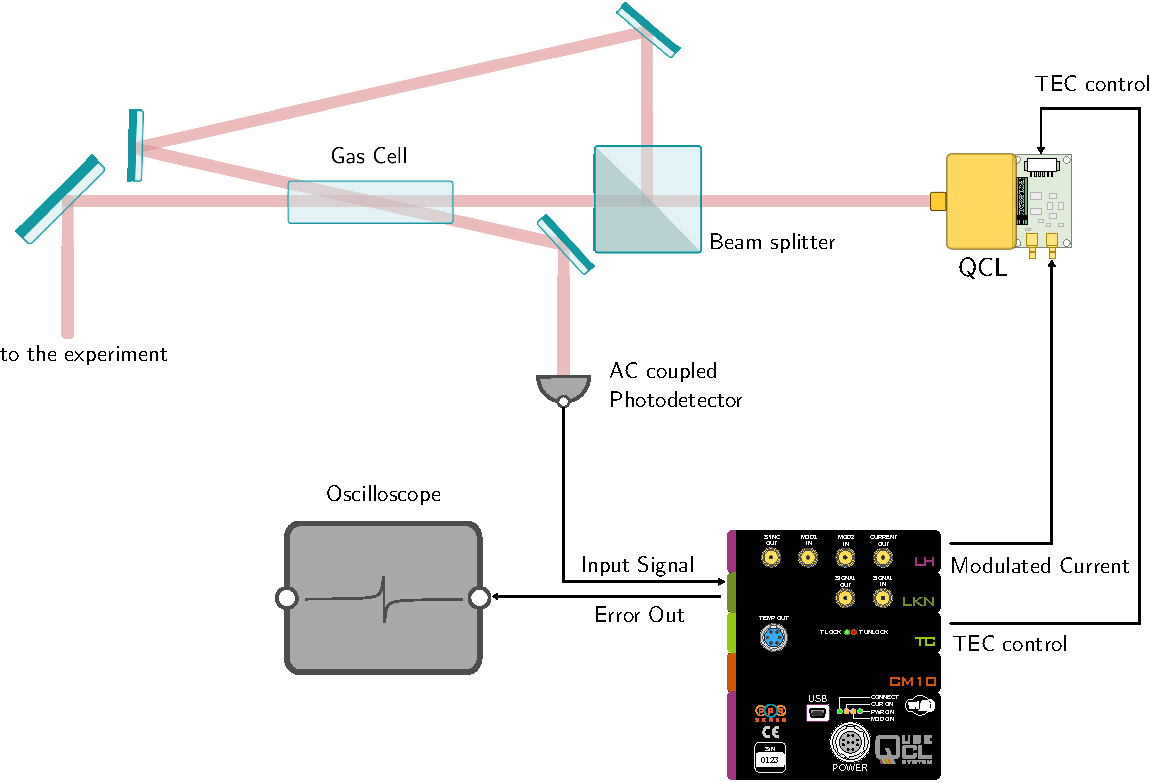
\includegraphics[width=12cm]{images/LKN_EXPERIMENT_DEMO.pdf}
\caption{spectroscopic line lock using LIA module}
\label{fig:spectroscopic-line-lock}
\end{figure}
\newpage
Using the lock-in module (LIA) installed on the \QubeModel  System, it is possible to directly acquire the spectroscopy signal from the photodetector and apply the correction to the laser for frequency locking.
In this configuration, the \QubeModel  is able to perform internally all the necessary operations to control the locking procedure:
\begin{itemize}
    \item[1.]Current modulation with frequency and amplitude control
    \item[2.]Signal demodulation with amplification and integration-time control
    \item[3.]Processing of the error signal by using a PID controller 
    \item[4.]Addition of the correction current directly to the laser bias current
\end{itemize}


The Qube Control Software allows to keep under control all the parameters for the optimization of the locking procedure.

\begin{figure}[H]
\centering
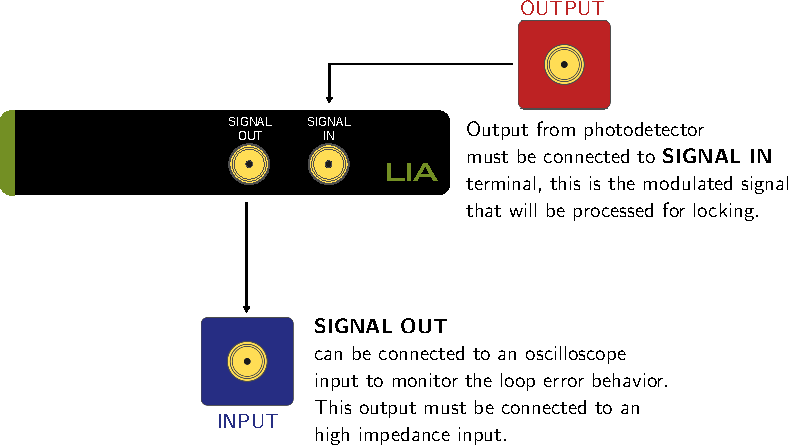
\includegraphics[width=12cm]{images/LIA_INPUT_EXPLANATION.pdf}
\caption{LIA terminals explanation}
\end{figure}




\newpage
\section{Offset phase lock with PLL module}

Frequency locking between two lasers is a technique for transferring the frequency and phase characteristics of a reference laser to a target laser.

It is commonly used in spectroscopic applications and in metrology.
\newline
The figure shows a possible optical scheme for an implementation of an offset phase lock between two Quantum Cascade Lasers anyway the \QubeModel  System can work with any type of diode laser.
\begin{figure}[H]
\centering
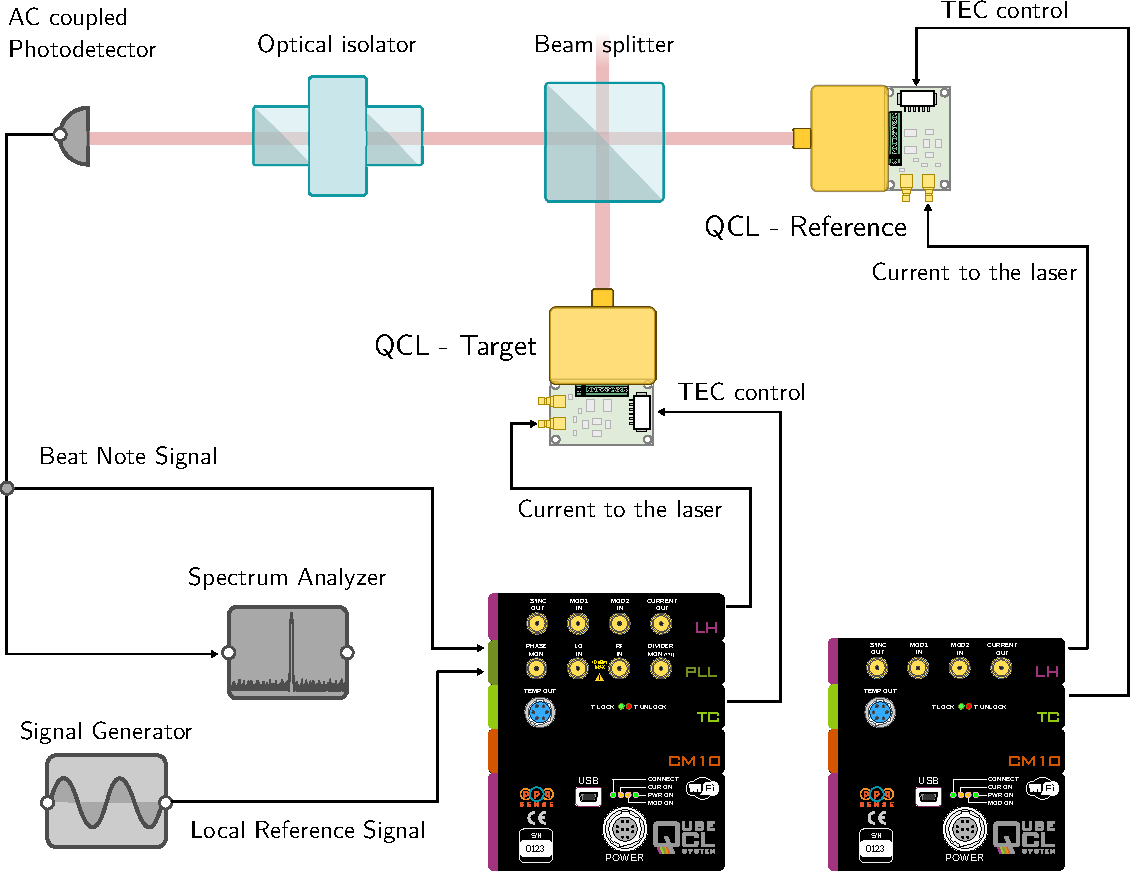
\includegraphics[width=12cm]{images/PLL_EXPERIMENT_DEMO.pdf}
\caption{PLL laser lock setup}
\end{figure}
The reference light is superimposed on the target light using a beam splitter.

The overlap of the beams is detected with a wide band photodiode and generates a beat signal at the frequency difference between the target light and the reference,
the beat-note frequency is usually in the hundreds of MHz.

The beat-note frequency is a function of the phase difference between the target light and the optical reference and it is constant only if the frequency difference between the target light and the reference light is exactly zero, any phase change will result in a variation of the signal.

To perform an offset lock, the beat note is mixed with a local RF reference  signal with frequency $\omega_{offset}$, 
at this point the signal obtained from this procedure will be constant only if the frequency difference between the target light and the optical reference is exactly $\omega_{offset}$, this is the final error signal used for offset frequency locking.

Using the PLL module integrated in the QuebeCL System, it will be sufficient to send the photodiode signal to the RF IN input and the module will add the correction signal directly to the laser current for frequency/phase stabilization, through the Qube Control Software it is possible to keep under control all the parameters for the optimization of the locking procedure.

\begin{figure}[H]
\centering
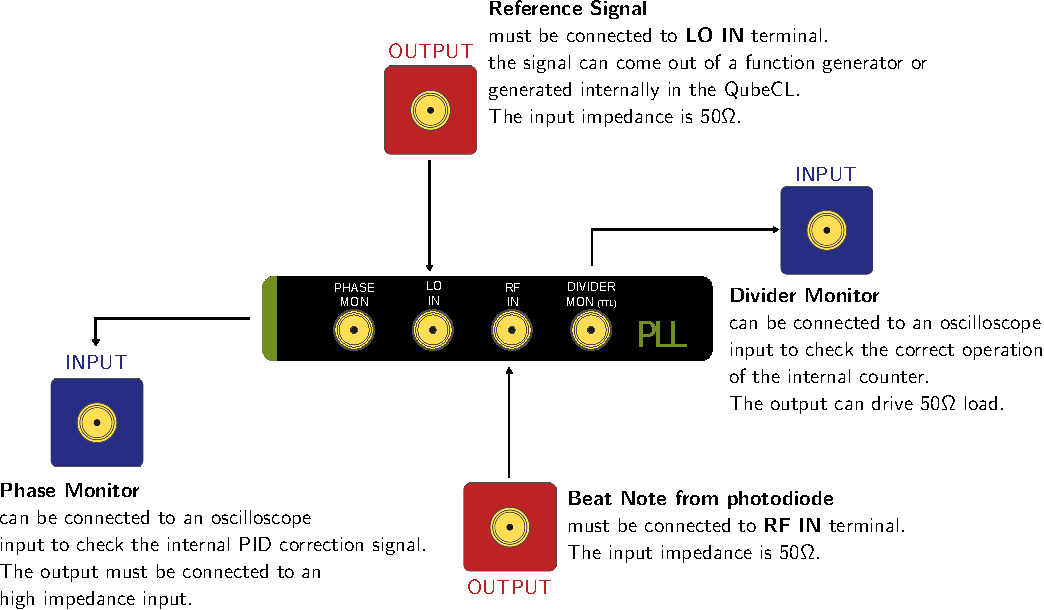
\includegraphics[width=12cm]{images/PLL_INPUT_EXPLANATION.pdf}
\caption{PLL terminals explanation}
\end{figure}


\newpage
\section{High finesse cavity lock with PDH module}

The Pound-Drever-Hall technique is a method to match the emitting optical frequency of a laser to a resonance of a Fabry-Perot cavity.
However stable the laser and cavity may be, both the length of the cavity and the frequency of the laser vary over time.
PDH locking technique uses the light reflected from the cavity to create an error signal that can be used to correct the laser frequency or change the length of the cavity so that they stay matched and transmission is maximized.

In the PDH technique the laser frequency is modulated, modulated light consists of a carrier frequency and two sidebands.
The light reflected from the cavity is measured using a fast photodetector, the reflected signal consists of the two unaltered sidebands together with an out-of-phase carrier component.
\newline
The photodetector signal is mixed with a local oscillator, which is in phase with the light modulation. After phase shift and filtering, the resulting electronic signal has a dispersive line shape that can be used as error signal for active stabilization.

For high-fineness cavities, the frequency spacing of the sidebands can be of the order of MHz, in this situation the modulation can be applied directly on the laser current, without the need for external electro-optical modulators.


\begin{figure}[H]
\centering
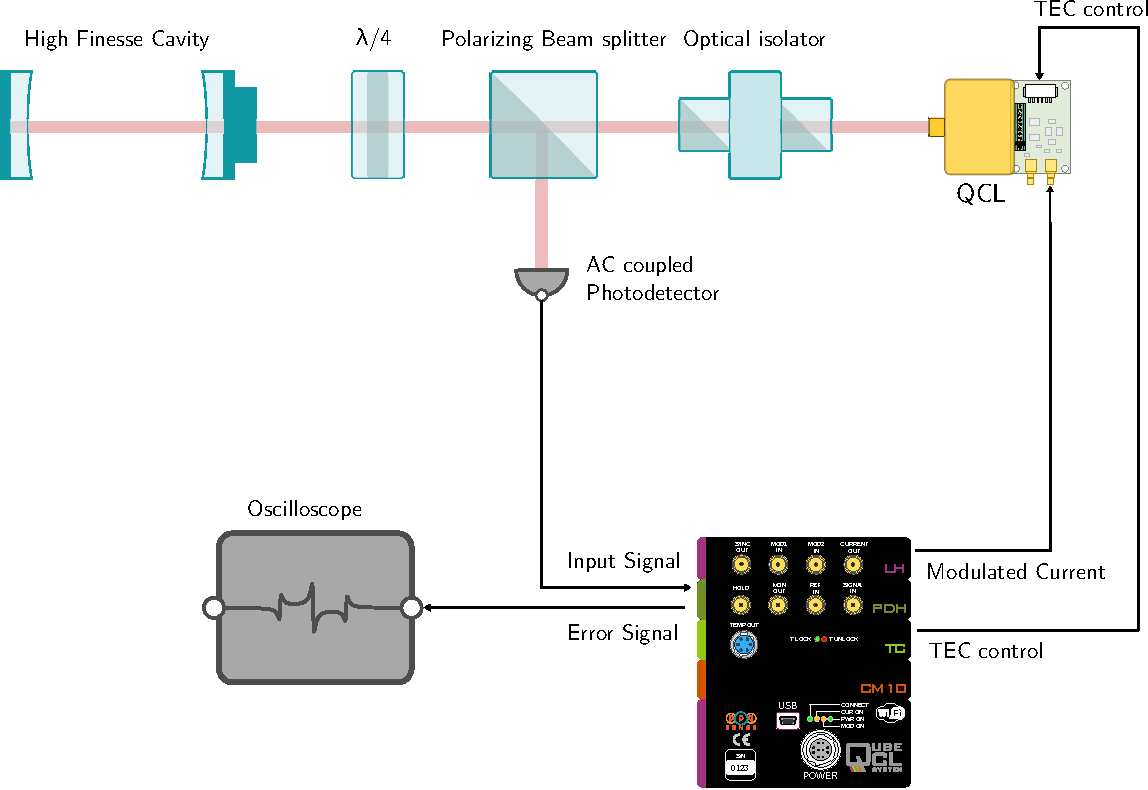
\includegraphics[width=12cm]{images/PDH_EXPERIMENT_DEMO.pdf}
\caption{PDH cavity lock setup}
\end{figure}

The PDH module accepts in input directly the signal coming from the photodiode, processes it and applies the correction to perform the lock directly on the laser current. The  Qube Control Software allows to keep under control all the parameters for the optimization of the locking procedure.

\begin{figure}[H]
\centering
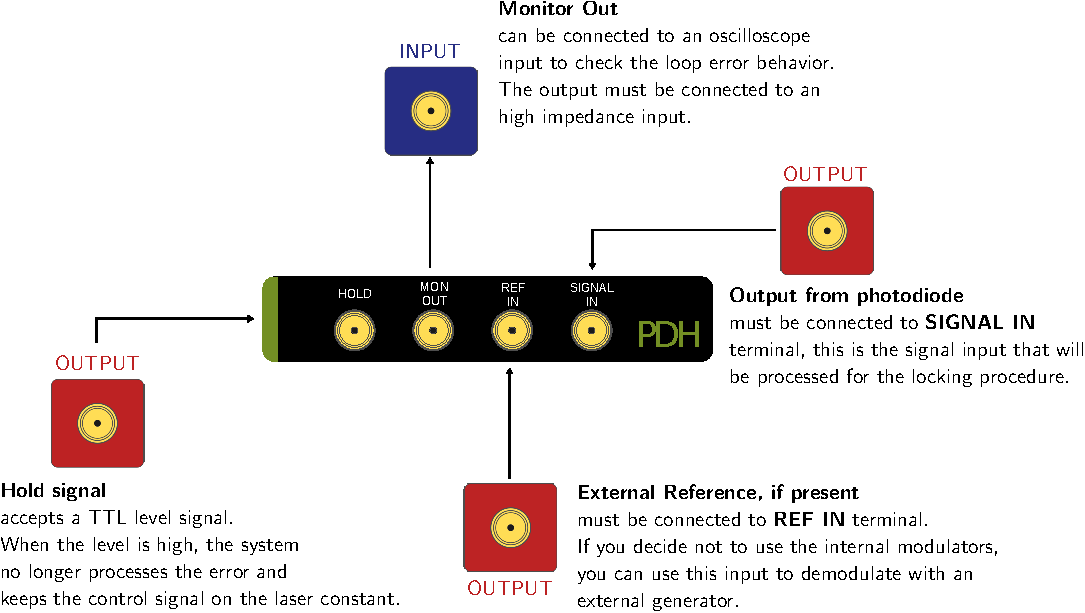
\includegraphics[width=12cm]{images/PDH_INPUT_EXPLANATION.pdf}
\caption{PDH terminals explanation}
\end{figure}


    \newpage

    \section{Customer support and useful contacts}

\paragraph{} The ppqSense staff can be reached for any problem or request concerning the \QubeModel  devices.
\newline To address any malfunctions or request help while working with our \QubeModel , please write an email to \textbf{qube.support@ppqsense.odoo.com}, our staff will reply to the raised ticket as soon as possible.
\newline To obtain quotations, support or updates concerning the purchase of our instruments, please write an email to \textbf{info@ppqsense.com}.

\paragraph{} All the available documentation concerning both the \QubeModel  and all our other products can be found on our website: \textbf{www.ppqsense.com}.
\newline The Technical Resources section of the website contains the user manuals, datasheets, brochures and application notes to help users working with the most advanced functionalities of the \QubeModel .

\paragraph{} \textbf{ppqSense s.r.l.} \newline Viale L. Ariosto 492/B \newline 50019, Sesto Fiorentino (FI) \newline Italy \newline +39 055 80 23 943

\begin{figure}[h]
    \centering
    
\includegraphics[width=5cm]{images/ppqSense_Logo.pdf}
    \label{logo_ppqsense}
\end{figure}
    \newpage

    \begin{versionhistory}
        \vhEntry{1.0}{2025.05.29}{LM}{First redaction.}
    \end{versionhistory}
\end{document}